% CREATED BY DAVID FRISK, 2016
\chapter{Introduction} 

The algorithm in question that we designed a custom GPU for is called sphere
tracing.\cite{Hart1996} So called since it uses spheres to incrementally
advance a ray in 3D space. The method of advancing rays incrementally is called
ray marching and is a particular subset of ray tracing.\cite{Whitted1980} Ray
tracing, then, is a way of wholly or partially rendering the world through
rays, cast from the eye of the observer into the scene.  Sphere tracing has
been around since at least as early as the late eighties and ray tracing as
early as the sixties.\cite{Hart1989,Appel1968} Since ray tracing traditionally
has been a more computation-intensive method compared to
scanlining\cite{Wylie1967} and as such it has generally seen more use in movie
production rather than in real-time applications.\cite{ref_needed?} 

%TODO(bjorn): Nån som är bätre än mig på detta får gärna skriva om denna delen
              %nedanför. låter inte proffsigt alls.

The advent of the programmable shader brought back the discussion of real time
ray marching to the forefront. which is where we caught on to it.
\cite{JamieWong2016} It still favours poorly compared to other techniques which
natrually begged the question if it would be able to compete in real time if
only the hardware for it was there.

\section{Sphere tracing} 

\begin{minipage}{0.6\textwidth} 

    At the base of the algorithm are the signed distance functions.
    $$\text{SDF}:\mathbb{R}^{3}\mapsto\mathbb{R}$$ The "distance" is the
    distance between a point and the closest point on the implicit surface
    $\text{SDF}^{-1}(0)$. The "signed" part refers to the distance being
    negated when measured inside of the surface.  If we define a ray $$r(s) =
    \vec{d} \cdot s + \vec{o}$$ where $\vec{d}$ is the normalized direction of
    the ray and $\vec{o}$ the origin, then $$\text{SDF}\circ r(s) = 0$$ means
    that the ray intersects a surface at exactly the distance $s$ from its
    origin.

\end{minipage} 
\hfill
\noindent
\begin{minipage}{0.3\textwidth}
    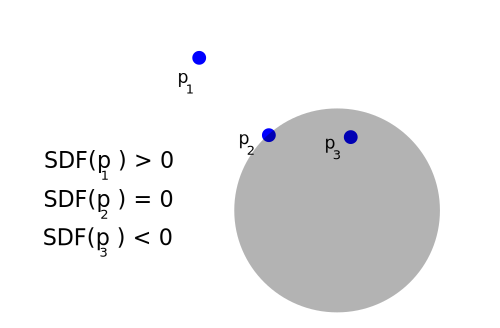
\includegraphics[width=\linewidth]{figure/SDF} 
\end{minipage}

\bigskip

Finding the surface can be done by iterating point by point from the origin
along the ray like below. $$p_{i+1} = p_i + \vec{d}\cdot \text{SDF}(p_i)$$ This is
repeated until $\text{SDF}(p_i) \leq \varepsilon$ for a given precision limit
$\varepsilon$. $\text{SDF}(p_i)$ is the furthest we can march the ray while
still be sure we don't overshoot any potential surfaces.  The direction of the
closest surface point is never known thus $\text{SDF}(p_i)$ can be interpreted
as a sphere bound, giving the algorithm its namesake. This ray marching is then
performed for each pixel of the screen reversely simulating the light rays from a
scene entering the lens of the onlooker.
	
	\subsection{Reflections and refractions}

                Once a point on a surface for a given pixel has been located
                new multiple rays can then be further marched to determine
                reflections, towards the scene's sources of light determening
                light and shadows, or through the object with an angle,
                simulating refractions. A lot of these depend on the surface
                normal which can be calculated by normalizing the aproximate
                gradient of $\text{SDF}(p)$. 
	
	\subsection{Textures}
		
                Texturizing could at least be done in two ways. The
                straightforward way would be to use the surface point coupled
                with an id-signature of the figure. After translating and
                re-scaling the point to the origin, it could then be directly
                looked up in a 1:1 3D texture as per its id. A more indirect
                but space-saving alternative could be to replace the last step
                with a sphere trace from the translated point along its surface
                normal\footnotemark out towards a simple wrapping geometry. The
                resulting surface coordinate could then along with the whole
                surface be transformed into a 2D flat plane mapping to a
                corresponding 2D texture. The texture and enclosing geometry
                again being variable according to the id of the figure.
	
\footnotetext{Or along the normal of the point.}

	\section{Hardware implementation}
